%  +---------------------------------+
%  | LaTeX template file for AES LAC |
%  +---------------------------------+
% This file is a modification of the template used for the
% AES Brazil.
% To be used with "aeslac.cls" version 1.0

%%
%% NOTE: This text file uses UNIX line feed conventions. When (human)
%% reading this file on other platforms, you may have to use a text
%% editor that can handle lines terminated by the UNIX line feed
%% character (0x0A).
%%

%%%%%%%%%%%%%%%%%%%%%%%%%%%%%%%%%%%%%%%%%%%%%%%%%%%%%%%%%%%
%
%  CARGADO DE LA CLASE
%
% La clase "aeslac.cls" carga automáticamente los siguientes paquetes:
%    hyperref, graphicx, color, times, y helvet.
% El paquete "graphicx.sty" es necesario para incluir imágenes,
% gráficos, etc. El uso de pdflatex requiere que el formato de las
% imágenes sea PDF, PNG, o JPG (no EPS).

% Para generar el documento en formato DVI, eliminar la opción 'pdfout'
% y ejecutar
% > latex template
% > bibtex template
% > latex template
%
% Para generar el documento en formato PDF ejecutar:
% > pdflatex template
% > bibtex template
% > pdflatex template

% Eliminar la opción "pdfout" si no se está usando 'pdflatex'.
% La opción "ams" carga los paquetes "amsmath", "amssymb" and "amsthm".
\documentclass
  [ams,pdfout]% opciones de la clase
	{aeslac}

%%%%%%%%%%%%%%%%%%%%%%%%%%%%%%%%%%%%%%%%%%%%%%%%%%%%%%%%%%%
%
% CARGADO DE PAQUETES
%
% Usar \RequirePackage en lugar de \usepackage
% Esto evita conflictos entre paquetes.

% Usar formato 8-bit UCS/Unicode Transformation Format
\RequirePackage[utf8]{inputenc}

% Para escribir el documento en español es necesario usar la opción
% "spanish" de "babel"
\RequirePackage[spanish]{babel}

% Usar caracteres extendidos
% Solo es necesario para escribir en portugués
\RequirePackage{textcomp}

%\let\oldcdot\cdot
%\usepackage{breqn}
%\let\cdot\oldcdot

\DeclareMathOperator*{\argmin}{argmin}

\begin{document}
% La página del título es construida en el ambiente "TitlePage".
% En ese ambiente se genera el título, los autores y
% sus respectivas afiliaciones y el resumen, en ese orden.
\begin{TitlePage}
	% El titulo es producido con el comando \Title.
	\Title{Alineación audio partitura en la flauta traversa}
	% \RunningTitle y \RunningAuthors son impresos en el
	% encabezado de cada página.
	\RunningTitle{Alineación audio partitura en la flauta traversa} % titulo corto
	% 2 o mas autores:
	% ("Autor1 y Autor2" para 2 autores.)
	% ("Autor1 et al." para 3 o mas autores.)
	\RunningAuthors{Juan P. Braga Brum et al.}
% Especificar autor y afiliación (con \Author y \Affil) para cada
% autor (en ese orden).
% Primer autor
	\Author
		[juanbragabrum@gmail.com]% email
		{Juan P. Braga Brum} % Nombre del autor (impreso en la página del titulo)
		\Affil
			[A]% clave (argumento opcional)
			{%
				Universidad de la República (UdelaR),
				Facultad de Ingeniería (FIng),
				Instituto de Ingeniería Eléctrica (IIE)\\
				Montevideo, 11300, Uruguay
			}
	\Author
		[wagner@smt.ufrj.br]
		{L. W. P. Biscainho}
		\Affil
			[B]% clave (argumento opcional)
			{%
				Universidade Federal do Rio de Janeiro (UFRJ), 
				Escola Politécnica (Poli),
				Departamento de Engenharia Eletrônica e de Computação (DEL)\\
				Rio de Janeiro, RJ, 21941-972, Brasil
}
	\Author
		[obudon@vera.com.uy]
		{Osvaldo Budón}
		\Affil
			[C]% clave (argumento opcional)
			{%
				Universidad de la República (UdelaR),
				Escuela Universitaria de Música (EUMus),
				Instituo de Ingeniería Eléctrica\\
				Montevideo, 11200, Uruguay
}	
	\Author
		[pcancela@fing.edu.uy]
		{Pablo Cancela}
		\Affilref[A]
	
	\Abstract{%
		Un sistema de alineación entre audio y partitura para señales de flauta traversa es presentado. 
		Para eso, un abordaje desde el material sonoro generado de la flauta traversa es realizado. 
		La comparación de desempeño de varias estrategias en la base de datos de flauta tradicional es realizada.
		La base de datos queda disponible para futuros trabajos en el área.
		 
		%
	}%
\end{TitlePage}
%
% Los títulos de las secciones se escriben usando mayúsculas
\section{Introducción}

La alineación entre audio y partitura es la asociación entre dos tipos de datos: muestras de audio digital y notación simbólica de música. Es un tema de investigación que ha captado la atención durante más de 30 años, de la comunidad científica en áreas como el Procesamiento de Audio, Machine Learning y Computer Music \cite{orio2003score}. El problema se puede dividir en dos grandes enfoques de resolución en \textit{online}\footnote{Refiere a análisis en tiempo real} y \textit{offline}, cada uno con aplicaciones diferentes y características propias de la estrategia utilizada.

El enfoque offline cuenta con toda la interpretación de la obra mediante un archivo de audio al momento de procesamiento, siendo posible analizar de forma no causal y lograr mayor precisión en la alineación partitura y audio. Se puede ver como el indexado de las muestras de audio según la información de la partitura. En otras palabras, asociar los eventos simbolizados en la partitura con las correspondientes muestras de audio de una grabación, como se esquematiza en la Figura \ref{fig:resultado_alineacion}. La resolución del problema offline tiene diversas aplicaciones de interés como los editores de audio inteligentes que acceden al audio a través de compases y notas de la partitura, búsquedas asistidas en grandes bases de datos a partir de fragmentos de notación músical, herramientas para el análisis automático de parámetros expresivos como son las dinámicas, variaciones de tempo, articulaciones, entre otros \cite{dannenberg2006music}.

\begin{figure}[h!]
\begin{center}
\includegraphics[width=0.4\textwidth]{imagenes/resultado_alineacion} 
\caption{Esquema conceptual de la alineación entre audio y notación simbólica.}
\label{fig:resultado_alineacion}
\end{center}
\end{figure} 


En cambio, la resolución del problema en tiempo real tiene como principal motivación transformar la interacción entre computadora-humano en una experiencia bidireccional, simulando el comportamiento de una interpretación de un músico con otro. En la literatura es usualmente denominado también como acompañamiento automático o músico sintético \cite{vercoe1984synthetic}. Tiene directa implicancia en la música electroacústica de medios mixtos, donde se combina el material sonoro generado por una computadora con la ejecución de instrumentos musicales.

Por otro lado, la flauta traversa es elegida por muchos compositores para la creación de música para medios mixtos\footnote{Música donde se combina el material sonoro generado por una computadora con la ejecución de instrumentos musicales.} (i.e. Música Electroacústica). Teniendo en cuenta que sistemas basados en algoritmos de alineación audio partitura tienen directa implicancia en esta corriente musical, el alcance del presente trabajo se acota a señales de flauta traversa. Dando lugar a la creación de una base de datos de flauta traversa para evaluación de algoritmos de alineación audio partitura que se hace pública para su uso con fines académicos.

Base de datos,
Experimentos,


%
\subsection{Flauta traversa}

Las técnicas para la generación de sonido con el instrumento se clasifican en dos grupos. Por un lado existen las técnicas tradicionales, que son las de uso común del instrumento, asociadas a la generación de música principalmente basada en alturas y duraciones. En complemento a lo anterior, los compositores y flautistas contemporáneos han definido una nueva clase de técnicas llamadas extendidas\footnote{El desarrollo de técnicas extendidas tiene estrecha relación con el desarrollo de la música electroacústica desde mediados del siglo xx. La síntesis electrónica y la manipulación electroacústica del sonido introdujeron en la creación musical nuevas sonoridades, que suministraron modelos para la experimentación sonora en la música instrumental}. Éstas, como su nombre lo indica, extienden las capacidades sónicas del instrumento generando material sonoro que va más allá del definido con alturas y duraciones. No es objetivo de esta sección hacer una descripción exhaustiva del material sonoro generado con las distintas técnicas, para eso existe extensa bibliografía \cite{piston1955orchestration,samuel2002study,dick1975other}. Por el contrario, presentar los aspectos relevantes para la comprensión de la naturaleza de las señales de flauta, y los desafíos que presentan las técnicas extendidas en áreas científicas de investigación con el \textit{Music Information Retrieval} (por su denominación en inglés).   


\subsection{Técnicas tradicionales}

Las técnicas tradicionales de la flauta son aquellas con las cuales el material sonoro ejecutado es definible mediante los parámetros de altura y duración. Como su nombre lo indica, las mismas refieren al uso tradicional de la flauta traversa y sus mecanismos de producción de sonido. Para comprender la naturaleza de las señales generadas con técnicas tradicionales se comienza identificando dos elementos esenciales: por un lado la producción de la excitación periódica, y en complemento a lo anterior el largo de la columna de aire. Además, se hace un esbozo de las características tímbricas detallando los modos de vibración del instrumento, y se finaliza dejando en claro las limitaciones en registro de la flauta traversa. 

\subsection*{Producción del sonido}

Existen dos procesos independientes que son los encargados de definir la nota que emite la flauta. Por un lado, la generación de la excitación periódica que pone a resonar la columna de aire y en complemento, el largo de la misma determinada por la configuración de las llaves presionadas por el instrumentista. 

Para poner en oscilación al instrumento, el flautista debe soplar superando en el interior de su boca la presión atmosférica. El trabajo\footnote{En su acepción como concepto de la Física.} necesario para subir la presión interna y acelerar el aire es la fuente de energía de entrada al instrumento, por lo que al intérprete se lo puede modelar como una fuente continua de energía. Sin embargo, las notas musicales se generan a partir de un movimiento oscilatorio. Estas fluctuaciones periódicas de energía son generadas a partir de la colisión del flujo de aire con el filo del agujero de la embocadura. En otras palabras, la turbulencia provocada por la colisión genera una onda viajera que se traslada a través del flujo de aire. Ésta es la que pone a resonar la columna de aire interior al tubo de la flauta. De esta forma, se genera entonces un sonido de naturaleza periódica denominado como nota musical.

Puesto a resonar el tubo, la frecuencia fundamental de la nota emitida depende estrictamente del largo de la columna de aire oscilatoria. Para el control de este parámetro, existen las llaves del instrumento (en la flauta moderna) que tapan o liberan los agujeros del tubo. Un agujero libre significa la imposición de presión atmosférica en ese punto de la columna de aire, definiendo de esta forma el largo de la misma.


\subsection*{Modos de Vibración}

Además de la mecánica de producción de sonido, es de relevancia mencionar aspectos tímbricos del sonido de la flauta. En la práctica, una configuración de llaves en el instrumento permite más de un modo de vibración\footnote{Refiere a las ondas estacionarias que un medio de propagación y sus características permiten.}, generando otras alturas musicales que se suman a la de frecuencia fundamental. Se tiene que para una columna de aire con largo determinado (i.e. posición de llaves determinada por el instrumentista) resonando en el interior del tubo, existe emisión simultánea de otras alturas musicales por encima de la de frecuencia fundamental. Éstas dan un sonido característico y se las denomina armónicos. En la Figura \ref{fig:espectrograma_armonicos} se observa el espectrograma de una señal de flauta donde se identifican visualmente la frecuencia fundamental con sus armónicos.


De forma teórica se pueden deducir los armónicos permitidos por la construcción del instrumento, modelándolo como un tubo cilíndrico con sus dos extremos abiertos. De esta forma, el modelo impone que la presión en los extremos sea la atmosférica, definiendo dos nodos\footnote{El nodo de una onda refiere, a un punto donde la variación de energía es nula a lo largo del período.} de presión. Por el contrario, en el interior del tubo la presión no está impuesta, siendo posible las variaciones de energía. De lo anterior, se deduce que la onda de mayor longitud que soporta las condiciones de borde\footnote{Las condiciones de borde refiere a la imposición de nodos de presión en los extremos del tubo cilíndrico.} tiene una longitud de dos veces la distancia entre los nodos de presión (en su forma matemática se escribe como $\lambda=2L$). De la misma forma, se deduce que existen otras longitudes de onda permitidas en este modelo, y se demuestra matemáticamente que cumplen $\lambda=2L/k$, con $k \in N$.

Por otro lado, la frecuencia del modo de vibración se calcula como la velocidad de propagación de la onda sobre la longitud de la misma, matemáticamente se expresa como $f=v/\lambda$. De la relación anterior se deduce en primer lugar, que la mayor longitud de onda provoca la altura más baja, que en el caso particular de la flauta es la frecuencia fundamental. En segundo lugar, que la estructura armónica de la flauta se puede expresar como $f_{i}=(i+1)f_{0}$, donde $i \in N$ y $f_{0}$ es la frecuencia fundamental en Hertz. 


\subsection*{Registro}

Por último, se especifican las notas musicales que son emitibles por la flauta traversa. Esta característica asociada al instrumento se denomina registro, y determina el rango de frecuencias posibles en el instrumento. La cota inferior del registro queda determinada por el pie elegido, para el caso de \textit{pie en $C$} el limite es el $C4$, por el contrario para \textit{pie en $B$} es el $B3$. Del otro lado, en la parte alta del registro, la flauta moderna alcanza notas superiores a $C7$, en particular $C\#7$ y $D7$ (observar Figura \ref{fig:registro_flauta}). La producción del sonido a partir de $A6$ se vuelve dificultosa, siendo posible para flautistas expertos \cite{samuel2002study}.

\begin{figure}[h!]
\begin{center}
\includegraphics[width=0.15\textwidth]{imagenes/registro_flauta} 
\caption{Registro de la flauta traversa. Se observa la cota inferior del registro para flauta con \textit{pie en $B$} y \textit{pie en $C$}.}
\label{fig:registro_flauta}
\end{center}
\end{figure} 


\subsection{Técnicas extendidas}

Con el afán de extender el lenguaje musical, los compositores contemporáneos\footnote{E.g. George Crumb (Estados Unidos, 1929), Helmut Lachenmann (Alemania 1935), Salvatore Sciarrino (Italia, 1947).} se han dedicado a explorar las capacidades sónicas de los instrumentos musicales. Para esto, se siguen procedimientos como la intervención\footnote{Denominado también como la preparación de instrumentos. Por ejemplo, el piano preparado de John Cage (Estados Unidos, 1912-1992) y la cabeza móvil en la flauta traversa (\textit{Glissando Headjoint} por su denominación original) de Robert Dick (Estados Unidos, 1950).} mecánica de instrumentos o la definición métodos no ortodoxos de ejecución. Es así, que en el caso particular de la flauta se ha derribado el mito de que la sonoridad del instrumento es limitada, y hoy en día existe un diccionario bien definido de técnicas reproducibles, denominadas extendidas\cite{dick1975other}.

No es objeto de esta sección el detalle exhaustivo de las técnicas extendidas para flauta traversa, mencionar los procedimientos de ejecución más extendidos en la flauta contemporánea. Algunas de las técnicas más conocidas se enlistan a continuación (se utilizan las denominaciones en inglés):

\begin{itemize}

\item \textbf{Flutter Tonguing:} Refiere a la generación del soplido con aleteo de la lengua. 
\item \textbf{Tongue Noises:} Ruidos con la lengua dentro de la embocadura. 
\item \textbf{Percussive Sounds:} Presión de las llaves de forma percusiva.
\item \textbf{Microtonal Inflections:} Inflecciones microtonales.
\item \textbf{Multiphonics:} Sonidos multifónicos (más de una nota a la vez con el instrumento).
\item \textbf{Cantar y tocar a la vez:} Como su nombre lo hace explicito la ejecución de dos alturas a la vez mediante el canto y el instrumento.

\end{itemize}

La exploración en la música contemporánea abarca también el control tímbrico y la calidad del sonido como un parámetro notado por el compositor. En esta línea, la ejecución de sonidos de banda angosta y banda ancha son muchas veces elementos buscados desde la composición. En el caso particular de la flauta, este nuevo material sonoro se ejecuta mediante el control de la embocadura\footnote{El término embocadura refiere al aparato de producción de la excitación de la columna de aire, en conjunto con la técnica de soplido.} así como la presión de aire. En el Capítulo \ref{cap:caso_de_estudio} se explora la capacidad de algunas técnicas computacionales en la extracción automática de la embocadura (i.e. detectar automáticamente el tipo de embocadura a partir de el análisis de las muestras de audio) con el objetivo de evaluar la capacidad de representación de algunas caracaterísticas clásicas en el material sonoro generado con técnicas extendidas. Como caso de estudio se utilizan grabaciones de la obra \textit{Aliento/Arrugas} (1998) del compositor contemporáneo Marcelo Toledo (Argentina, 1964). 

\subsection{Alcance y desarrollo de la publicacion}
%
\section{Alineación Audio-Partitura}

La resolución del problema de alineación entre audio y partitura es generalmente dividida en dos etapas. En primer lugar, ambas representaciones de la misma pieza musical (i.e. grabación y notación simbólica) deben ser llevadas a un espacio de características donde puedan ser comparables, usualmente llamado como representación intermedia. Ésta transformación genera a la salida dos series temporales de vectores con la misma dimensión. Para posteriormente definir la correspondencia punto a punto entre la representación del audio y la notación simbólica mediante algún algoritmo de alineación.


En 1984 en la conferencia ICMC (\textit{International Computer Music Conference}) aparecen las primeras publicaciones que dieron comienzo a esta linea de investigación. Ambas se basaban en una estrategia de \textit{string matching} para generar la alineación en tiempo real. Dannenberg con la publicación \cite{dannenberg1984line} describía un sistema basado en programación dinámica y una representación simbólica de la música de alto nivel. Para esto la partitura y eventos midi generados por el instrumentista en tiempo real eran comparados y alineados. Por otro lado, Vercoe publicó en \cite{vercoe1984synthetic} su intérprete sintético (\textit{Synthetic Performer} por su denominación en inglés) para acompañamiento de flauta traversa. La estrategia se basaba en representar audio y partitura como una lista de alturas (\textit{pitches} por su denominación en inglés). Como en ese entonces los detectores de pitch no eran ni lo suficientemente rápidos ni robustos para trabajar en tiempo real, la estimación de pitch desde el instrumento se hacía con la colocación de llaves que enviaban señales midi al sistema con la posición de los dedos. Posteriormente, en 1990 se introdujo \textit{EXPLODE} por parte de Puckette \cite{puckette1990explode}. Varias piezas musicales para medios mixtos\footnote{En Echo de Philippe Manoury para soprano y computadora, tal vez es de las más conocidas.} fueron escritas para interpretación basada en este sistema. Si bien la experiencia fue exitosa, los compositores debían sacrificar aspectos musicales para asegurar el correcto funcionamiento del sistema a la hora de dar un concierto. 

\subsection{Dynamic Time Warping}

Para la definición del problema de alineación de forma matemática, supóngase que se tienen dos series temporales $\vec{X}\in\mathbb{R}^{M\times D}$ y $\vec{Y}\in\mathbb{R}^{N\times D}$, donde $D$ es la dimensión del vector de características, y $M$ y $N$ el largo de las mismas respectivamente. La alineación está dada por dos secuencias, dígase $p, q \in \mathbb{N}^{L}$, que definen la correspondencia punto a punto entre $\vec{X}$ e $\vec{Y}$. Por lo que, de forma matemática se dice que $\vec{X}[p[i]]$ y $\vec{Y}[q[i]]$ están alineados. Para encontrar la correspondencia entre series se debe resolver el siguiente problema de minimización:

\begin{equation}
p,q = \argmin_{p,q} \sum_{i=1}^{L} d(\vec{X}[p[i]],\vec{Y}[q[i]]) 
\end{equation}

Este problema de minimización, con algunas restricciones sobre las secuencias $p$ y $q$, es resolube con el algoritmo denominado como DTW (\textit{Dynamic Time Warping} por su denominación en inglés). Esta es una técnica consolidada para la alineación de series numéricas con fuerte correspondencia temporal, como es el caso de señales de voz hablada\cite{rabiner1978considerations,sakoe1978dynamic}. También es el caso, en el problema de alineación entre audio y partitura como se vió en la sección \ref{sec:estado_del_arte} dedicada al estado del arte. El tipo de restricciones definen variantes de DTW que son detalladas más adelante en la presente sección.

Por otro lado, DTW es una técnica de programación dinámica por lo que se divide el problema en muchos subproblemas cada uno de los cuales contribuye al cálculo de la distancia total de forma acumulativa. El primer paso es el cómputo de $D$ la matriz de similaridad, que depende estrictamente de la distancia utilizada, el cálculo se define matemáticamente como


\begin{equation}
\label{eq:matrizsimilaridad}
D[i,j] = d(\vec{X}[i],\vec{Y}[j])
\end{equation}
donde $D[i,j]$ tiene $M\times N$ elementos donde representan la distancia entre todos los pares de puntos de las series temporales $\vec{X}$ e $\vec{Y}$.  


El segundo paso corresponde al computo de $C$ la matriz de costo acumulada. El cálculo se hace de forma recursiva como muestra la siguiente ecuación (esta no es la única forma de calcular la matriz de costo como se verá más adelante), 

\begin{equation}
\label{eq:matrizcosto}
C[i,j] = min\left\lbrace  
\begin{array}{ll}
C[i,j-1] + w_h\cdot D[i,j]\\
C[i-1,j] + w_v\cdot D[i,j]\\
C[i-1,j-1] + w_d\cdot D[i,j]
\end{array}
\right.
\end{equation}
donde $C[i,j]$ es el costo del camino menos costoso, desde el punto $(1,1)$ hasta el $(i,j)$. Además $C[1,1]=d(\vec{X}[1],\vec{Y}[1])$. Los valores $\vec{w}=(w_h,w_v,w_d)$\footnote{Notar que los subindices refieren respectivamente a dirección horizontal, vertical y diagonal} son factores de penalización, donde valores mayores que $1$ desalientan movimientos en la dirección correspondiente. A efectos de los cálculos en la presente tesis, siguiendo las recomendaciones de \cite{sakoe1978dynamic}, se utiliza $\vec{w}=(1,1,2)$ sin penalizar ninguna dirección. 

Luego que se completa el cómputo de la matriz $C$, se busca el camino de menor costo obteniendo la alineación entre series dada por $p$ y $q$. Éste se encuentra haciendo recursión hacia atrás desde $C[M,N]$ hasta $C[1,1]$. El algoritmo se compone de decisiones locales óptimas bajo el supuesto de que el resultado será un mínimo global. En concreto, se comineza desde $C[M,N]$ evaluando todas las celdas vecinas buscando el mínimo, éste se agrega al comienzo del camino y de forma sucesiva el procediemitno finaliza al llegar a $C[1,1]$. En la Figura \ref{fig:matrizcosto} se observa a modo de ejemplo una matrices $C$ y $D$. 


Por otro lado en las ecuaciones \ref{eq:dist_coseno_ok} y \ref{eq:dist_euclideana} se definen de forma matemática dos distancias de uso común en la literatura para la resolución del problema y las usadas en la presente tesis.


\begin{equation}
\label{eq:dist_coseno_ok}
d_{coseno}(\vec{X},\vec{Y}) = 1 - \frac{\vec{X}\cdot\vec{Y}}{\lVert\vec{X}\rVert_{2}\lVert\vec{Y}\rVert_{2}}
\end{equation}

\begin{equation}
\label{eq:dist_euclideana}
d_{euclideana}(\vec{X},\vec{Y}) = \lVert \vec{X} - \vec{Y} \rVert_{2}
\end{equation}


\subsection{Restricciones sobre el cámino de mínimo costo}
\label{sec:restricciones}

Las restricciones sobre el camino acotan el universo de posibilidades en la búsqueda del mínimo, disminuyendo el costo computacional en el cálculo de la alineación. La elección correcta de estas restricciones está asociada al conocimiento a priori del problema que se quiera resolver, es así que se pueden aplicar sin atentar contra el resultado final. En lo que sigue se hará mención solamente de las restricciones que fueron aplicadas para los experimentos de la tesis, para más detalle se recomienda el libro clásico de L. Rabiner et al \cite{rabiner1993fundamentals} o el más reciente de M. Muller \cite{muller2007information}.
  
En el caso partícular de alineación entre audio y partitura existe una correspondencia directa entre notación simbólica y las grabaciones de audio. Es claro si se tiene en cuenta que el músico ejecuta la pieza mediante la lectura de la partitura. Ésta característica de las series temporales en el problema planteado, permiten aplicar las restricciones que se especifican a continuación:

\begin{itemize}
\item \textbf{Limites}: Los limites de la alineación deben cumplir la siguiente condición: $p[1] = q [1] = 0$ y $p[L] = M, q[L] = N$. Es razonable suponer que la grabación empieza y termina con la ejecución del cominezo y el final de la partitura.
\item \textbf{Monotonicidad}: Las secuencias deben cumplir: $p[i+1] \geq p[i]$ y $q[i+1] \geq q[i]$. Teniendo en cuenta que la ejecución de la partitura se hace en una lectura direccionada (i.e. de izquierda a derecha) sin cambios a la dirección contraria parece una restricción acorde. 
\item \textbf{Continuidad}: Por último se impone: $p[i+1] \leq p[i] + 1$ y $q[i+1] \leq q[i] + 1$.  Suponiendo que el intérprete no realiza ningún salto en la lectura de la partitura durante la ejecución no debería resultar en el descarte de una solución válida. 
\item \textbf{Ventana de ajuste}: Teniendo en cuenta que las fluctuaciones temporales entre audio y partitura nunca serán excesivas se puede limitar el cómputo de la matriz de costo a una ventaja de ajuste. Existen varias formulaciones en la literatura, en la presente tesis se trabaja con la denominada de Paliwal en honor a su autor \cite{paliwal1982modification}. Matemáticamente se escribe como: $|p[i]\frac{N}{M}-q[i]|<r$, donde el término $r$ es usualmente denominado como radio y define el tamaño de la ventana de ajuste. Notar que la ecuación presenta el factor de escala $\frac{N}{M}$ que permite penalizar de la misma forma ambas dimensiones. 
\item \textbf{Pendiente}: Si la pendiente no se limita el mejor cámino puede contener fragmetos puramente horizontales o verticales, permitiendo saltearse fragmentos enteros de la partitura o grabación. Esto puede ser favorable en casos donde el intérprete se saltea una parte de la partitura, o ejecuta un material sonoro que no se encuentra escrito. Por el contrario, puede ser desfavorable en casos donde haya correspondencia directa entre partitura y ejecución. Existen varias estrategias para limitar la pendiente del mejor cámino, los expermientos realizados en la presente tesis utilizan las propuestas en \cite{sakoe1978dynamic}. A continuación se las define matemáticamente: 

%\begin{itemize}

%\item $P=0$:\begin{equation*}
%	\label{eq:matrizcosto}
%	C[i,j] = min\left\lbrace  
%	\begin{array}{ll}
%	C[i,j-1] + D[i,j]\\
%	C[i-1,j] + D[i,j]\\
%	C[i-1,j-1] + 2\cdot D[i,j]
%	\end{array}
%	\right.
%	\end{equation*}

%\item $P=0.5$:\begin{equation*}
%	\label{eq:matrizcosto}
%	C[i,j] = min\left\lbrace  
%	\begin{array}{ll}
%	C[i-1,j-3] + 2\cdot D[i,j-2] + D[i,j-1] + D[i,j]\\
%	C[i-1,j-2] + 2\cdot D[i,j-1]+ D[i,j]\\
%	C[i-1.j-1] + 2\cdot D[i,j]\\
%	C[i-2,j-1] + 2\cdot D[i-1,j]+ D[i,j]\\
%	C[i-3,j-1] + 2\cdot D[i-2,j] + D[i-1,j] + D[i,j]
%	\end{array}
%	\right.
%	\end{equation*}

%\item $P=1$:\begin{equation*}
%	\label{eq:matrizcosto}
%	C[i,j] = min\left\lbrace  
%	\begin{array}{ll}
%	C[i-1,j-3] + 2\cdot D[i,j-2] + D[i,j-1] + D[i,j]\\
%	C[i-1,j-1] + 2\cdot D[i,j]\\
%	C[i-3,j-1] + 2\cdot D[i-2,j] + D[i-1,j] + D[i,j]
%	\end{array}
%	\right.
%	\end{equation*}

%\item $P=2$: \begin{equation*}
%	\label{eq:matrizcosto}
%	C[i,j] = min\left\lbrace  
%	\begin{array}{ll}
%	C[i-2,j-3] + 2\cdot D[i-1,j-2] +2\cdot D[i,j-1] + D[i,j]\\
%	C[i-1,j-1] + 2\cdot D[i,j]\\
%	C[i-3,j-2] + 2\cdot D[i-2,j-1] + 2\cdot D[i-1,j] + D[i,j]
%	\end{array}
%	\right.
%	\end{equation*}

%\end{itemize}

\end{itemize}


\subsection{Estado del arte}

Existen diversas implementaciones de sistemas de alineación audio partitura con DTW, en la publicación \cite{orio2001alignment} una estructura espectral de picos es generada a partir de la partitura y es utilizada para el cálculo de distancia con las ventanas de audio analizadas. Aseguran que esta metodología es aplicable a señales polifónicas logrando mejores resultados y mayor robustez que las técnicas basada en extracción de pitch. Por otro lado en \cite{dannenberg2006music} se propone la utilización de DTW con extracción de características basadas en la representación tiempo frecuencia denominada como Chromagrama, este mismo sistema es presentado para la resolución del problema de \textit{Music Retrieval} en grandes bases de datos. Dixon en la publicación \cite{dixon2005live} es el primero en proponer una variante de DTW para la resolución del problema en tiempo real con la información disponible a cada instante, sacrificando desempeño del algoritmo. Además, en \cite{gagnon2007high} el camino optimo de alineación es calculado a partir de información de alto nivel como es chroma y una estimación de la duración y ritmo local a partir de la señal de análisis. 

\begin{table}[!ht]
\caption{Resultados de la competencia Mirex en Real-time  Audio to Score Alignment.}
\label{tab:Mirex}
\vspace*{10pt}
\centering
\small
\begin{tabular}{ll}
\textbf{Autor (Año)}	&	\textbf{Resultado}\\ \hline
Francisco J. Bris Peñalver (2017)     & 94\%   \\
Francisco J. Rodriguez Serrano (2016) & 97\%   \\
Francisco J. Rodriguez Serrano (2015) & 95\%   \\
Chunta Chen* (2014)                   & 91\%   \\
Julio J. Carabias Orti (2013)         & 86\%   \\
Julio J. Carabias Orti (2012)         & 83\%   \\
Kosuke Suzuki (2011)                  & 67\%   \\
\end{tabular}
\end{table}


Un salto cualitativo en los resultados del MIREX (observar tabla \ref{tab:Mirex}) fue logrado por el algoritmo implemetado por J. Carbias y detallado en la publicación\cite{carabias2015audio}. El sistema está separado en dos etapas: una etapa de procesamiento y a continuación la de alineación. En la primera etapa se hace la síntesis de la notación simbólica y mediante el análisis se obtienen patrones espectrales asociados a cada unidad de la partitura. Estos son aprendidos desde el audio generado por la síntesis, mediante la factorización espectral basada en NMF (\textit{Non-Negative Matrix Factorization} por su denominación en inglés). En la segunda etapa la descomposición espectral de la magnitud del espectrograma es realizada con los patrones aprendidos previamente resultando en una matriz de distorsión, que es utilizada como matriz de costo para el cómputo de DTW de forma online. La alternativa presentada por FJ Rodriguez Serrano\cite{rodriguez2017tempo}, que actualmente tiene el mejor resultado en la competencia, define el estado del arte. El algoritmo esta basado en el de J. Carabias donde el cómputo de la alineacíon se hace con DTW incorprorando información del tempo de la interpretación, mejorando notoriamente los resultados.


\section{Metodología}
Enventanado

Extracción de contenido musical
	B3aB8 CQT
	Normalización
	12 bins Chroma

Codificación de la partitura
	Silencio
	Armónicos

Síntesis

Distancia Coseno


\section{Experimentos}

Este capítulo está dedicado a la evaluación de desempeño de la solución planteada en la base de datos de flauta traversa. Se comienza evaluando la influencia de los parámetros de representación intermedia en el resultado de alineación. Se evalúan además distintas restricciones en el cámino óptimo de alineación de DTW. A continación, se hace una comparación de la estrategia de codificación de notación simbólica propuesta aquí, frente a la síntesis como paso intermedio. Para finalizar se hace una comparación con un algoritmo desarrollado por terceros. Todos los experimentos son realizados en el presente capítulo se realizan con la base de datos construída en el marco de la tesis. 

\subsection{Medidas de desempeño}
\label{sec:medidas_desempeno}

Para la evaluación de desempeño como se recomienda en la publicación \cite{orio2003score} se utilizan dos medidas, la tasa de aciertos y la precisión\footnote{Definida en este caso como una medida de desfasaje temporal entre las anotaciones y el resultado de la alineación.}. La primera cuantifíca la cantidad de notas bien identificadas, como porcentaje del total. Por otro lado, la precisión es el promedio del desfasaje de las notas bien identificadas con respecto al ground truth.

A la salida de la etapa de alineación se obtiene una lista como la representada en la Figura \ref{fig:datos_tabla}. Ésta es comparada con el ground truth correspondiente. Siendo $u(t_u)$ la altura del resultado de la alineación (i.e. frecuencia representada en midi) y $v(t_v)$ la del ground truth, en los tiempos $t_v$ y $t_u$ respectivamente, se definen los aciertos como los puntos que cumplen $|t_v-t_u|<tol$, si $u(t_u)=v(t_v)$. Por otro lado, la precisión matemáticamente se define como $\frac{\sum{|t_u-t_v|}}{N}$ siendo $N$ el largo de $v$ (i.e. la cantidad de notas en el ground truth). Para los cálculos del presente capítulo se definió la tolerancia $tol=200ms$ como se sugiere en la publicación \cite{orio2001alignment}.

\begin{figure}[h!]
\begin{center}
\includegraphics[width=0.4\textwidth]{imagenes/datos} 	
\caption{Ejemplo del resultado de etapa de alineación. Se observa la serie temporal representada como comienzo, altura y duración de las notas musicales.}
\label{fig:datos_tabla}
\end{center}
\end{figure}

\subsection{Base de datos de flauta tradicional}


Características

Kaggle

\subsection{Resultados}
Comparación

\begin{figure}[h!]
\begin{center}
\includegraphics[width=0.5\textwidth]{imagenes/comparacion} 	
\caption{Arriba, tasa de aciertos en función de la tolerancia. Abajo, precisión en forma de \textit{boxplot} para el caso $tol=200ms$. Aclaración: AA refiere a Alturas Absolutas y CA a Clases de Altura.}
\label{fig:datos_tabla}
\end{center}
\end{figure}


Por Obra

\begin{table}[!ht]
\caption{Tasa de aciertos por obra.}
\label{tab:por_obra}
\vspace*{10pt}
\centering
\small
\begin{tabular}{ll}
\textbf{Obra}	&	\textbf{Resultado}\\ \hline
Allemande     & 96\%   \\
Syrinx & 86\%   \\
Density 21.5 & 80\%   \\
Sequenza I & 70\%   \\
\end{tabular}
\end{table}


%%%%%%%%%%%%%%%%%%%%%%%%%%%%%%%%%%%%%%%%%%%%%%%%%%%%%%%%%%%
%
% EJEMPLO DE BIBLIOGRAFÍA
%
% para generar la bibliografía ejecutar "bibtex template"
\bibliographystyle{aes} % estilo aes.bst
\bibliography{bib} % archivo de bibliografía en formato bibtex
%
\end{document} 
